\documentclass[11pt]{article}

\usepackage[a4paper,margin=2.5cm]{geometry}
\usepackage{graphicx}
\usepackage{float}
\usepackage{booktabs}

\title{HPC: Labwork \#3}
\author{Nguyen Trong Minh}
\date{Tuesday, September 30, 2026 \\ SonTG}

\begin{document}

\maketitle

\section{Implementation}

The first step is to understand the input shape, since we want to use 2D threads to convert the image, we don't need to flatten it to 1D anymore as we did in labwork 3.
We can directly process the 2D image, we split the image into patches, then process each patch with a block in the grid of GPU. 

Because we use 2D grid in GPU now, the block size and grid now become a tuple. I experimented with multiple values for block size, ranging from 8x8 to 32x32, the limit is here because 64x64 > 1024 (max number of threads).
Now the image is in shape [width, height, channel], we need to access each pixel in that format too. However, the grid x-y value is reversed, so we need to do img[y,x,c].

The rest is to execute the conversion similar to labwork 3 and measure the time.

\section{Output Images}

Both implementations produce the same grayscale result. The output arrays are reshaped back to the original image dimensions before they are saved as PNG files.

\begin{figure}[H]
    \centering
    \begin{minipage}[t]{0.48\textwidth}
        \centering
        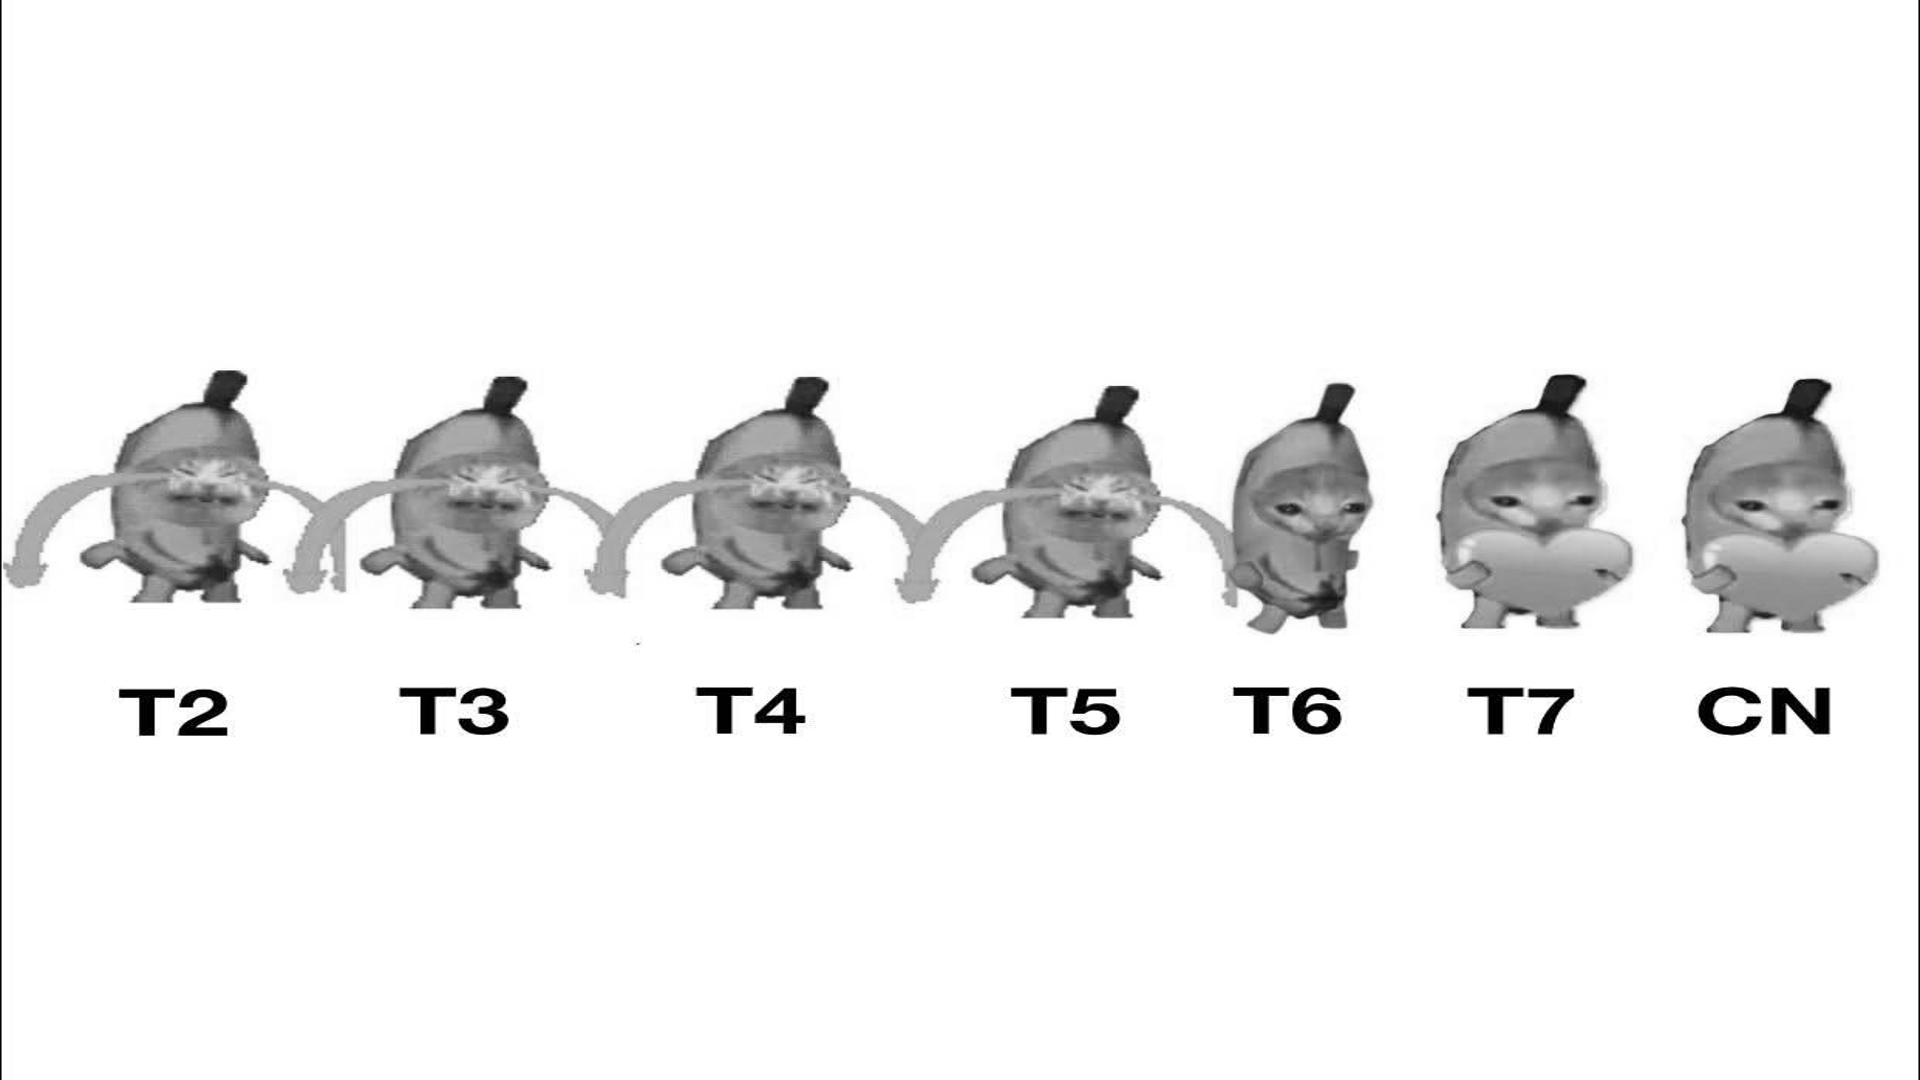
\includegraphics[width=\linewidth]{cpu_grey.png}
        \small CPU output
    \end{minipage}
    \hfill
    \begin{minipage}[t]{0.48\textwidth}
        \centering
        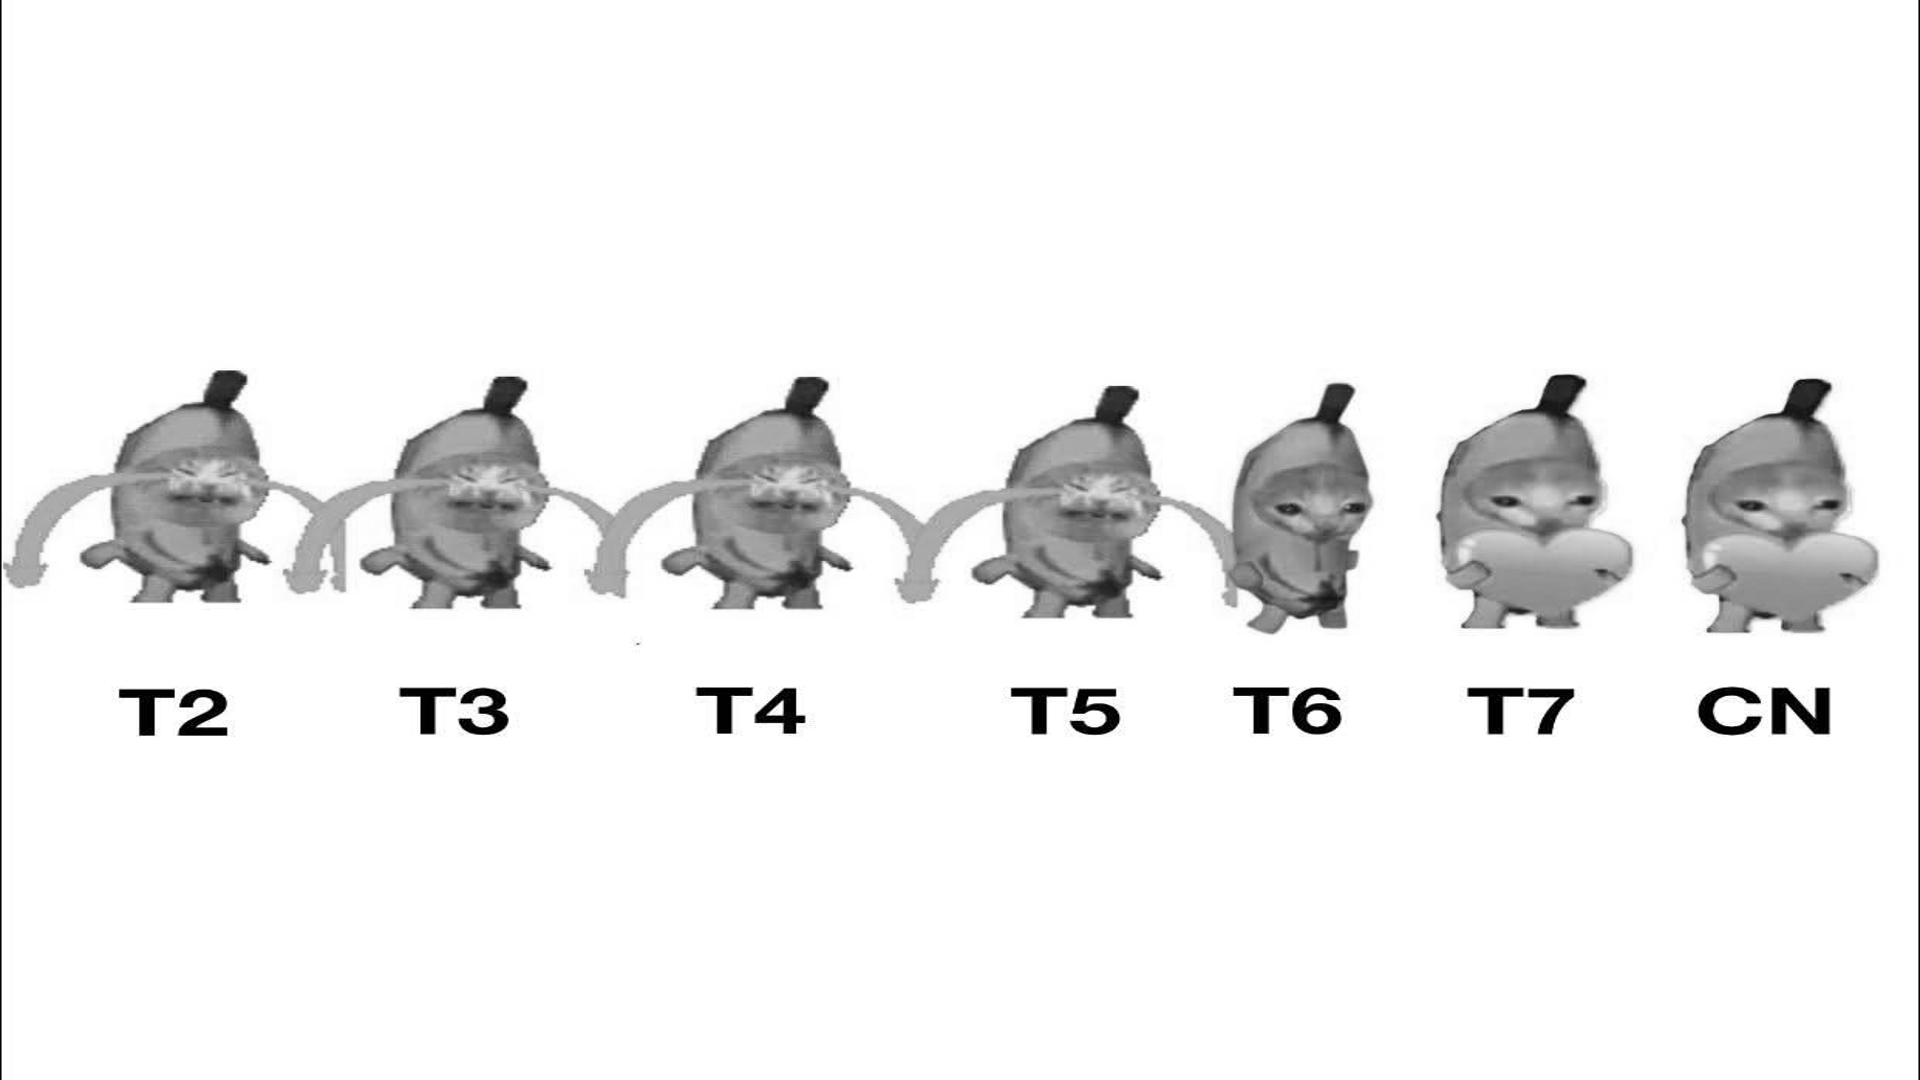
\includegraphics[width=\linewidth]{gpu_grey.png}
        \small GPU output
    \end{minipage}
    \caption{Grayscale images generated by the CPU and CUDA implementations.}
    \label{fig:outputs}
\end{figure}

\section{Result}

I resized the image to 1920x1080 and ran each block configuration 20 times, then took the average, because a single run is only around 0.5 ms and the result changes a lot between runs. To compare with labwork 3, I also ran the 1D kernel again with the same number of threads per block as the 2D shapes (64, 128, 256, 512 and 1024 threads). The result is shown in Table~\ref{tab:timing} and Figure~\ref{fig:timing}.

\begin{table}[H]
    \centering
    \begin{tabular}{lcc}
        \toprule
        Block size (x $\times$ y) & Threads per block & Execution time (ms) \\
        \midrule
        $8 \times 8$   & 64   & 0.612 \\
        $16 \times 8$  & 128  & 0.613 \\
        $8 \times 16$  & 128  & 0.605 \\
        $32 \times 8$  & 256  & 0.615 \\
        $16 \times 16$ & 256  & 0.618 \\
        $8 \times 32$  & 256  & 0.605 \\
        $32 \times 16$ & 512  & 0.625 \\
        $16 \times 32$ & 512  & 0.624 \\
        $32 \times 32$ & 1024 & 0.679 \\
        \midrule
        Best 1D (64 threads)  & 64 & 0.449 \\
        CPU                   & -- & 1850 \\
        \bottomrule
    \end{tabular}
    \caption{Average execution time of the 2D kernel for each block size, compared with the best 1D kernel and the CPU.}
    \label{tab:timing}
\end{table}

\begin{figure}[H]
    \centering
    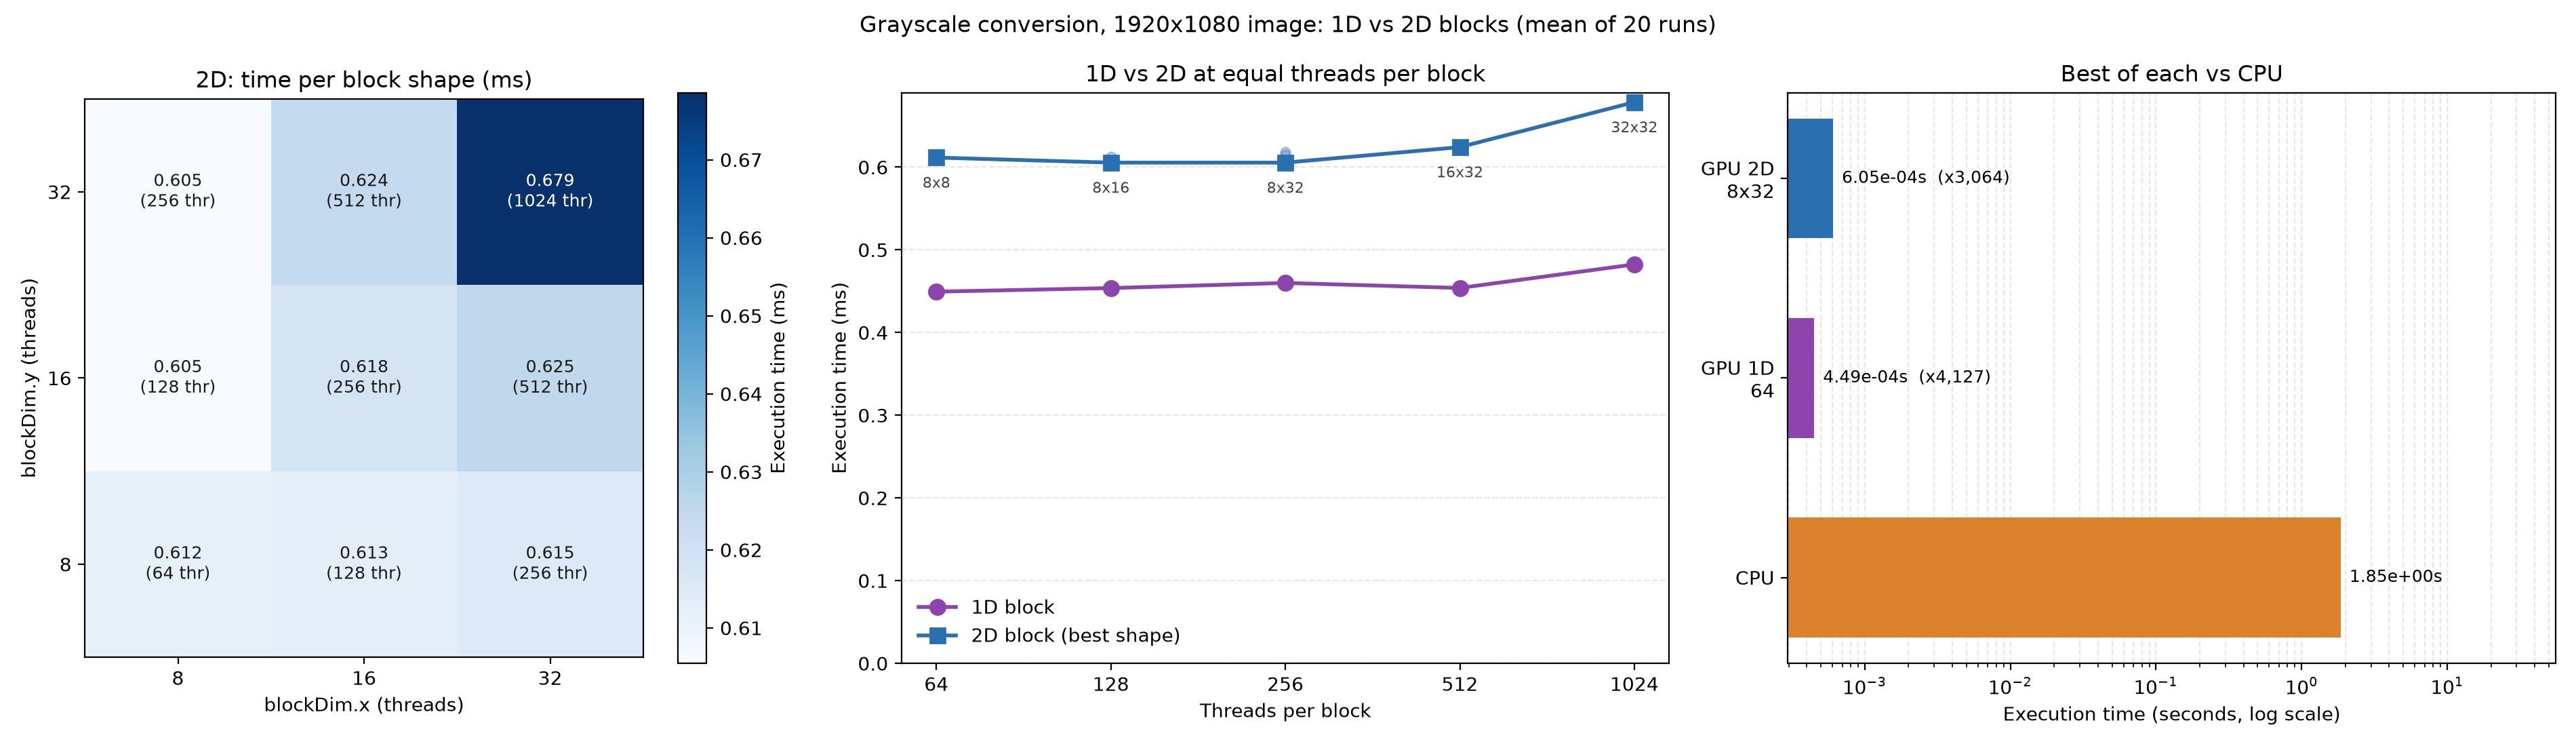
\includegraphics[width=\textwidth]{execution_time.png}
    \caption{Left: 2D kernel time for each block shape. Middle: 1D and 2D kernel time with the same number of threads per block. Right: best 1D, best 2D and CPU on a logarithmic scale.}
    \label{fig:timing}
\end{figure}

For the 2D kernel, the block shape does not change the time much. Most shapes are between 0.605 and 0.625 ms, which is less than 4\% difference, so I think most of it is just noise. The only clear outlier is $32 \times 32$ at 0.679 ms. With 1024 threads in one block, the GPU has less flexibility to schedule blocks on each streaming multiprocessor, so it is a bit slower. The 1D kernel also becomes slower at 1024 threads, so this behaviour is the same in both versions.

The surprising part is that the 1D kernel is faster than the 2D kernel. At every number of threads per block, 1D takes around 0.45 to 0.48 ms, while 2D takes around 0.60 to 0.68 ms, so 1D is about 25\% faster. My guess is that the 2D version does more work per thread: it computes two indices instead of one, and accessing \texttt{img[y, x, c]} on a 3D array needs more address calculation than \texttt{img[tidx, c]} on a 2D array. Since the grayscale conversion itself is very cheap, this extra indexing becomes a big part of the total time. The image is stored row by row in memory in both cases, so using 2D blocks does not give better memory access here.

Compared with the CPU (1.85 s), the best 2D configuration is about 3,000 times faster and the best 1D configuration is about 4,100 times faster. Same as labwork 3, the CPU version uses a Python loop, so this speedup is much bigger than it would be against an optimized CPU implementation.

\section{Conclusion}

Using 2D blocks makes the code closer to the shape of the image: we don't need to flatten the image, and each thread directly gets its (x, y) pixel. However, for grayscale conversion it does not make the program faster. The 1D kernel from labwork 3 is still about 25\% faster, and the block shape of the 2D kernel only matters when it gets to 1024 threads per block. The main things I learned in this labwork are that the grid and block are now tuples in (x, y) order, that x is the column so the image must be accessed as \texttt{img[y, x, c]}, and that the grid size needs to be rounded up, so a bounds check is needed for threads that fall outside the image. 2D blocks are probably more useful for problems where a thread needs its neighbour pixels, like blurring or convolution.

\end{document}
